\section{Extended Discussion}
\label{sec:extended-discussion}

\subsection{Additional Findings}

\paragraph{Vision Remains a Fundamental Limitation.} Community observations consistently identified vision as the primary failure mode: ``Claude's vision is beyond fixing with a prompt---it barely knows what up and down are.'' This suggests that game-playing benchmarks will continue to challenge AI systems until vision-language integration improves substantially. Concurrent independent work comparing Gemini 3 Pro and 2.5 Pro on Pokémon Crystal~\citep{zhang2025gemini3playspokemon} corroborates this finding, reporting that vision-related errors remained a dominant failure mode across model generations despite improvements in reasoning capability.

\paragraph{Frontier vs.\ Open-Source Performance Gap.} Our baseline evaluation (Figure~\ref{fig:track1_baselines}) reveals that frontier models significantly outperform open-source alternatives in direct prompting, with Gemini 3 Flash achieving 71\% GXE compared to 29\% for Gemma3-1B without a harness. However, the PokeChamp harness substantially narrows this gap: Gemma3-1B with a harness reaches 53\% GXE, demonstrating that architectural support can partially compensate for raw model capability. This finding has practical implications for benchmark accessibility---researchers without frontier model access can still achieve meaningful results through careful harness design. The comparison also validates Pokémon as an OOD evaluation: if models had seen extensive Pokémon training data, we would expect the performance gap between model scales to be smaller, as smaller models would have relevant cached knowledge. Instead, the gap reflects genuine reasoning capability differences that a harness can only partially bridge.

\paragraph{Model Behavior Diversity.} Different model families exhibited distinct failure patterns:
\begin{itemize}
    \item Claude models showed ``memory corruption cascades''---once false information entered context, they followed incorrect paths for extended periods
    \item Gemini models exhibited ``roadblock'' behavior---oscillating between contradictory goals when facing conflicting objectives
    \item GPT models demonstrated excessive plan commitment---persisting with suboptimal strategies for hours/days
    \item Qwen models exhibited ``computational paralysis''---entering recursive damage calculation loops and getting stuck verifying basic type matchups (``water vs fire?'') while the battle state evolved. This failure mode is striking: \textit{in high-stakes sequential decision-making, extended deliberation can be catastrophic}
\end{itemize}

\paragraph{Chain-of-Thought Visualization Enables Failure Diagnosis.} We deployed a live ladder stream that visualizes LLM chain-of-thought synchronized with battle state. This revealed failure modes invisible to outcome-only metrics. Figure~\ref{fig:cot_visualization} shows Gemma-3-12B vs Qwen-3-14B on Gen 9 OU: while Gemma articulates strategy and executes decisively, Qwen's reasoning trace shows real-time ``panic''---recursive verification loops that consume the decision window. Without CoT visualization, Qwen's poor performance would appear as generic ``weak play'' rather than a specific, diagnosable pathology.

\begin{figure}[h]
    \centering
    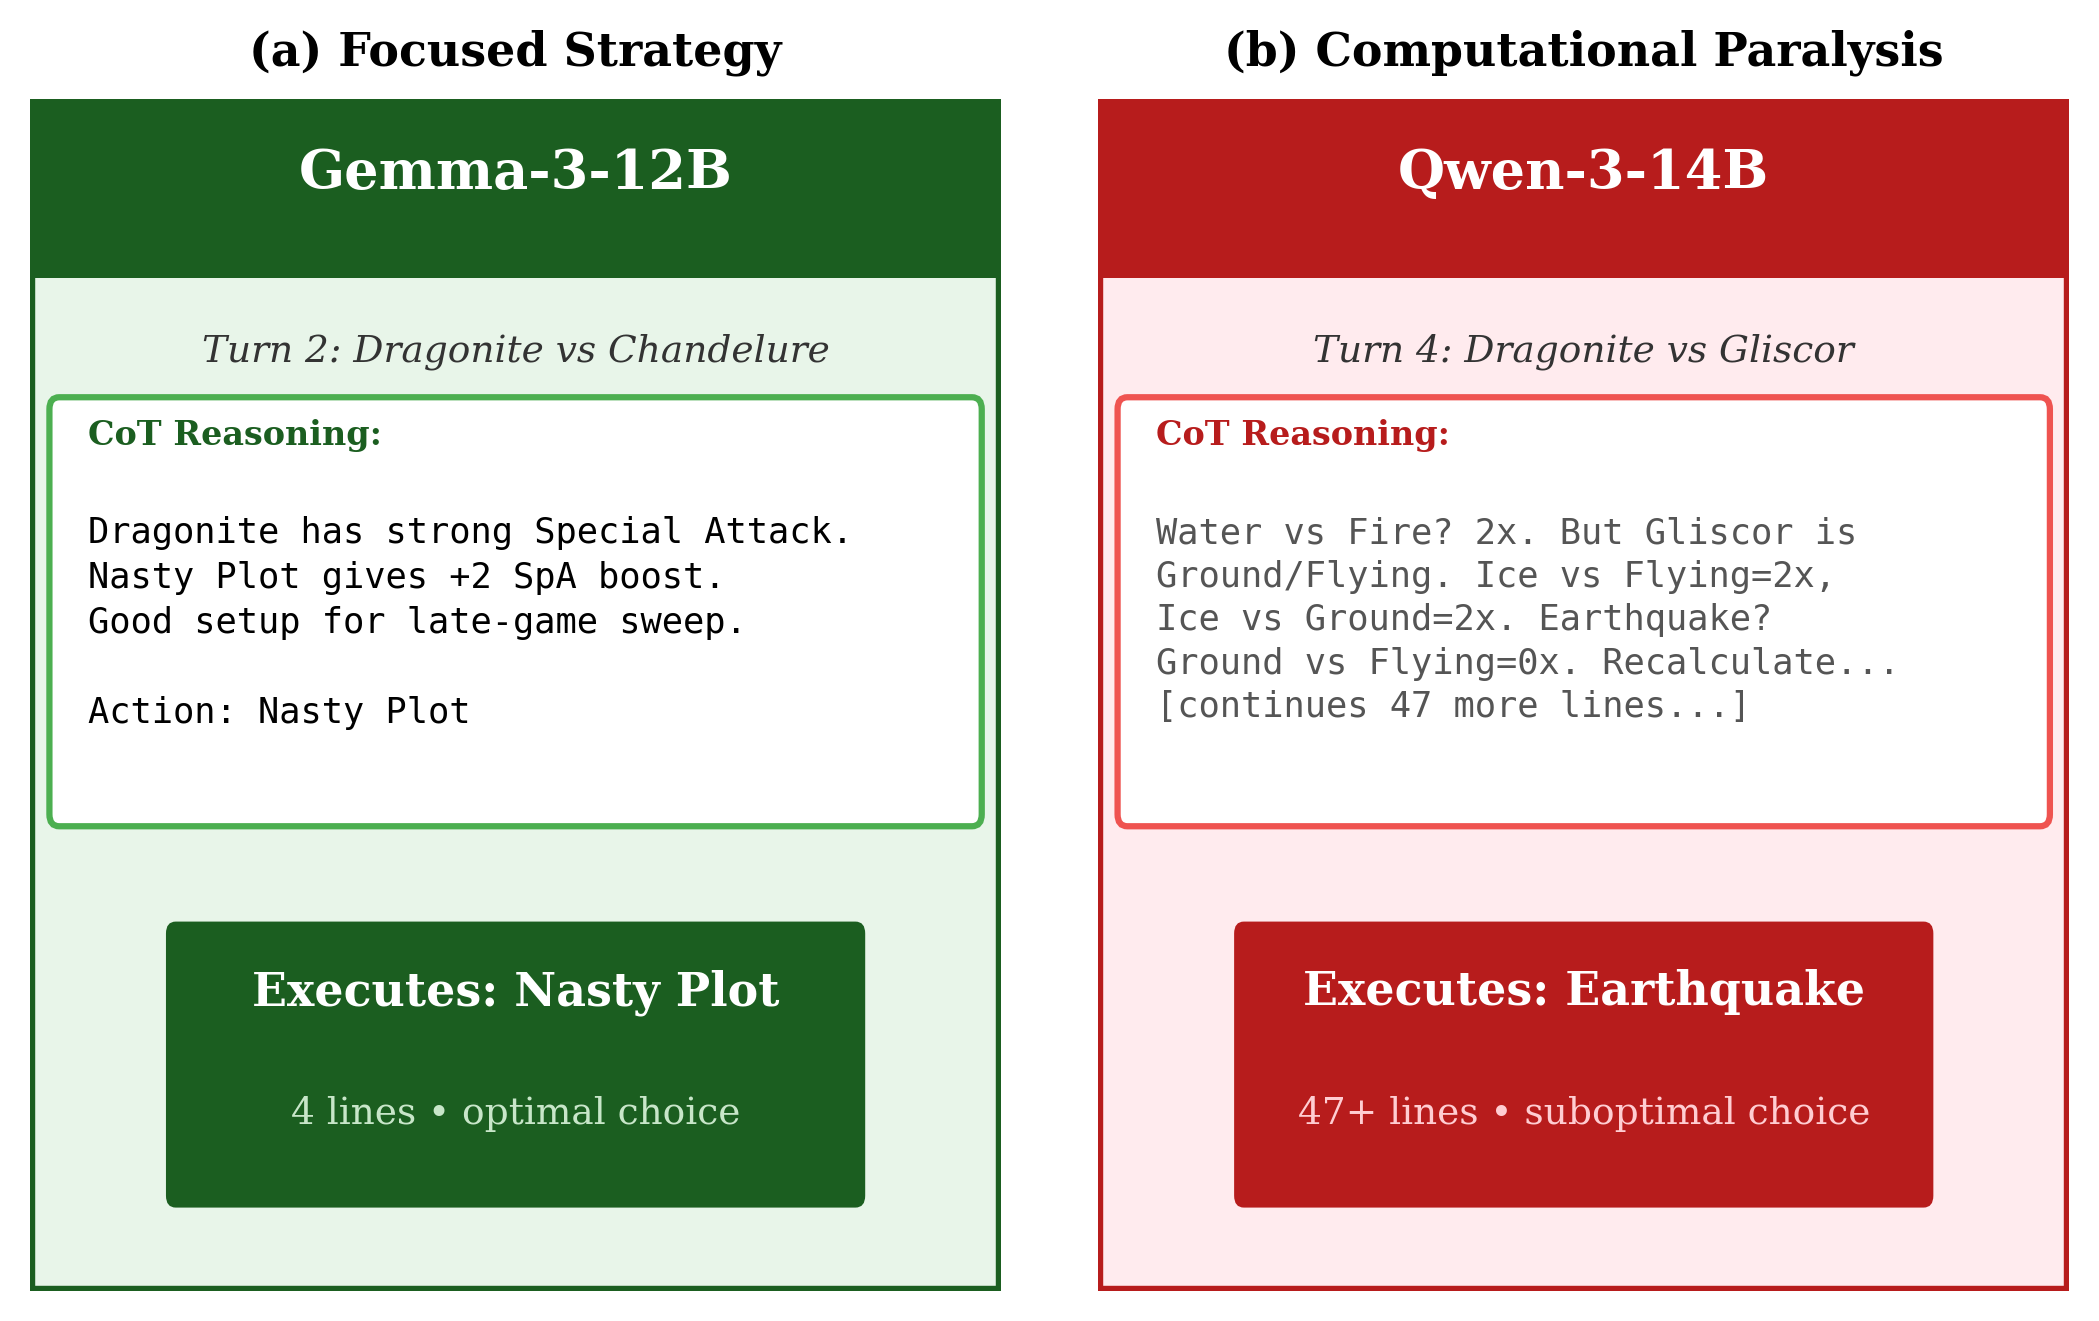
\includegraphics[width=0.95\linewidth]{figures/cot_visualization.png}
    \caption{\textbf{Chain-of-Thought Visualization Reveals Failure Modes.} Screenshots from our live ladder stream showing synchronized CoT reasoning during a Gen 9 OU battle between Gemma-3-12B (a) and Qwen-3-14B (b). In Turn 2, Gemma articulates a brief strategic assessment (``boosting Special Attack will be beneficial'') and executes Nasty Plot. By Turn 4, Qwen's reasoning trace fills the panel with recursive damage calculations---enumerating type matchups, computing exact damage ranges, and deliberating between moves---exhibiting the ``computational paralysis'' described in the text. This failure mode is invisible to win/loss statistics alone.}
    \label{fig:cot_visualization}
\end{figure}

\subsection{Broader Impact}


\subsubsection{Beyond Pokémon: From Game Agents to Coding Agents}

An unexpected outcome of the X Plays Pokémon has been the transfer of harness techniques to other domains. The modular context engineering harness that emerged as essential for game-playing agents has influenced the design of autonomous coding agents. Systems like Claude Code now incorporate similar harness patterns: persistent memory across sessions, hierarchical planning for complex tasks, and structured perception of codebases. Recent develops have entirely overlapped with autonomous gaming agents as coding agents have been used in 24/7 loops with the ``Ralph Wiggum'' extension and ``OpenClaw''. This convergence suggests that game-playing benchmarks serve as verifiable benchmarks for developing autonomous agent capabilities that transfer to practical applications.
